\chapter{Definición  del Espectro}

\begin{resumen}

En el siguiente capítulo se aborda el formalismo matemático que enmarca la definición del espectro de las señales cardiacas de esta \nombreDoc, y el cual se encuentra publicado en \cite{Requena13b}. La motivación del capítulo es desarrollar la teoría que conecta el espectro de la señales cardiacas, con su dinámica espacio-temporal de las señales cardiacas.

A lo largo del capitulo se plasman los diferentes conceptos necesarios para el análisis espectral, como la auto-correlación de las fuentes y señales cardiacas. Y mediante el análisis multivariante, se estudian los mecanismos para la estimación del espectro que conllevan a los mapas de \acf{DF} y de \acf{PF}. Por último, se abordan los efectos de sistemas de electrodos sobre el espectro de las señales.


Para terminar, se aborda los mapas de (\ac{DF}), como ejemplo de análisis espectral. en donde se expone la relación entre las características del sistema de electrodos, utilizados para estimar la actividad local del miocardio, y el ancho de banda del espectro resultante.

Los resultados teóricos, presentes en este capitulo, derivan en el análisis e
interpretación del espectro de señales cardiacas y los efectos del sistema
de electrodos, que se abordan en los próximos capítulos

NOTAS llega hasta la descripción de la correlación de voltajes  y la definición de tipos de fuentes se toma del articulo

\commentDir{ ... }

\end{resumen}


\section{Introducción}

% En el estudio de la fibrilaciones cardiacas, por medio de \ac{ECG}, se observan
% trazas muy irregulares de la señal captada, y por lo tanto, tradicionalmente se
% han descrito dichas arritmias complejas como aleatorias  y desorganizadas.
% Pero el análisis espectral, técnica ampliamente utilizada en el estudio de
% señales cardiaca, a permitido cuantificar la organización espacio-temporal del
% sustrato cardiaco durante la fibrilación. Con el uso de la teoria de la dinámica
% no lineal y gracias al desarrollo de técnicas de mapeo optico y eléctrico, se ha
% spropuesto que la fibrilación puede tener algun grado de regularidad
% espacio-temporal \cite{Hoekstra95, Jalife00}.
%
%
% De esta forma, las caracteristicas espectrales de señales cardiacas, se han
% propuestos como índices experimentales para la detección de \ac{VF} \cite
% {Barro89}, para cuantificar el grado de organización espacio-temporal de la
% \ac{AF} \cite{Everett01a} y para predecir el éxito de
% descargas de desfibrilación \cite{Strohmenger97, Eftestol00, Jekova04}.
% Adicionalmente con los mapas de \ac{DF} se han podido observar un grado de
% regularidad durante la \ac{AF} tanto en animales \cite{Skanes98,
% Mandapati00, Mansour01} como en humanos \cite{Sanders05, Atienza06}.
%
% Se observa, el análisis espectro de las señales cardiaca, viene en
% constante crecimiento. Sin embargo, aùn sigue siendo difusa la relación entre el
% espectro de señales cardiacas y la dinámica espacio-temporales de las fuentes
% cardíacas subyacentes. por lo cual en este capítulo se presenta  el formalismo
% matemático que sustenta la investigación el espectro de la actividad eléctrica
% del corazón.
%

% Los procesos estocásticos nos permiten modelar aquellos sistemas multivariantes,
% en tiempo y espacio. De esta manera, gracias a las herramientas estadisticas, se
% puede estudiar como se comportan señales variantes en el tiempo, que de otra
% forma serian muy dificiles de tratar. Los modelos estocásticos son fundamentales
% para el análisis espectral de señales bioeléctricas, y en general en señales
% discretas que se analizan en un tiempo finito. De esta formas, tanto la
% autocorrelación con la densidad espectral de potencia, son habitualmente muy
% utilizadas para describir procesos estocásticos de segundo orden. Con los
% estadisticos de segundo orden, por lo tanto, es posible describir patrones,
% tales como la periidicidad y la coherencia de las señales
% \cite{Requena08}. Siguiendo un enfoque de análisis de la señal multivariante, a
% lo largo de este capítulo, se identifica la relación entre el
% espectro de las señales cardiacas, la dinámica espacio-temporal de las fuentes
% cardíacos, y las características de los sistemas de captación de la actividad
% cardiaca.
%
%

\subsection{Variable Aleatoria}\label{subs:varaleatoria}

% Una variable aleatoria, como función medible que asigna un número real a cada
% posible resultado del espacio muestral de un experimento aleatorio, se puede
% caracterizar por medio de su probabilidad de ocurrencia. De esta forma, la
% función de distribución ${F(x)}$  es una descripción de las probabilidades
% asociadas a los posibles valores de la variable aleatoria.
%
% Por tanto, toda variable aleatoria tiene asociada una función de distribución
% ${F(x)}$, tal que ${F(x)=P(X \leq x)}$. Para variables aleatoria continua, la
% distribución de probabilidad viene descrita por una función de densidad
% ${f(x)}$. en donde, ${f(x)= dF(x)/dx}$. Asi mismo,  para las variables
% aleatorias discretas relacionamos la función de distribución con la función de
% densidad como ${F(x)= \displaystyle\sum_{x_i \leq x }f(x_i)}$.
%
% Un proceso estocástico es una sucesión infinita de variables aleatorias que
% evolucionan en el tiempo. Por lo tanto, al dependen del un tiempo $t$  la
% función de distribución da lugar a ${F(x,t)=P(\mathbf{x}(t) \leq x)}$.
% Por lo que, la función de densidad de $x(t)$ es $f(x,t)=
% \partial{F(x,t)}/\partial{x}$ \cite{Papoulis91}.
%
%
\subsection{Correlación de Señales}\label{subs:corresignal}

% Siendo $\mathbf{x}(t)$, un proceso estocasticos real y $\mathbf{x}(t_1)$,
% $\mathbf{x}(t_2)$, dos valiables aleatorias, se define, $\mathbf{R}(t_1,t_2)$,
% la autocorrelación de $\mathbf{x}(t)$ como \cite{Papoulis91}:
%
% \begin{eqnarray}\label{eq:autocorrelation}
% 	\mathbf{R}(t_1,t_2)=E{\{ \mathbf{x}(t_1)\mathbf{x}(t_2) \}}
% \end{eqnarray}
% Donde $E$ es la media estadistica. De esta manera, se define la autocorrelación
% de un procesos $\mathbf{x}$, real o complejo, como la media estadistica del
% producto de $\mathbf{x}(t_1)\mathbf{x}^*(t_2)$, donde la máxima correlación se
% obtienen cuando $t_1=t_2$.
%
% Cuando se tiene dos procesos estocasticos $\mathbf{x}(t)$ y
% $\mathbf{y}(t)$,se habla de corelación cruzada $\mathbf{R}_{xy}(\tau)$. como
% \cite{Requena08}:
%
% \begin{eqnarray}\label{eq:correlation}
% 	\mathbf{R}_{xy}(\tau)=E{\{ \mathbf{x}(t-\tau)\mathbf{y}(t) \}}
% \end{eqnarray}
% De esta forma, la correlación es la operación básica para la búsqueda de
% patrones por emparejamiento. como se expone en \cite{Requena08} el ruido blanco,
% $W(t)$, es un porcesos estocástico particular cuya función de autocorrelación es
% $\mathbf{R}(\tau)= \delta(\tau)$, donde $\delta(\tau)$ es la función delta de
% Dirac, y lo que indica es que las variables aleatorias que conforman $W(t)$
% no estan correlacionadas entre si.
%

\subsection{Correlación de Vectores}\label{subs:correvector}

% Un procesos vectorial, de $n$ dimensiones, es una familia de $n$ procesos
% estocasticos. Por lo tanto, un proceso estocástico vectorial es un
% vector cuyas componentes son procesos estocásticos escalares \cite{Requena08}.
%
% Se extienda la definición de la correlación de dos señales, sección
% \ref{subs:corresignal}, a los procesos vectoriales, al realizar para cada par de
% procesos escalares  definidos por el producto vectorial de dos procesos
% vectoriales, como se expone en \cite{Requena08}. La correlación de vectores es la correlación cruzada de los
% componentes del vector que dan como resultado las matriz de correlación
% cruzada.
%
% Si $\mathbf{V}_n(t)$ y $\mathbf{W}_n(t)$ son dos procesos vectoriales  de $n$
% dimensiones, $\{v_1, v_2, v_3, \ldots v_n\}$ y  $\{w_1, w_2, w_3, \ldots
% w_n\}$ los respectivos procesos estocasticos. Entonces, acorde con la
% la ecuación \ref{eq:correlation}, decimos que la correlación cruzada entre dos
% componentes de $\mathbf{V}_n(t)$ y $\mathbf{W}_n(t)$, esta definida
%
%  \begin{eqnarray}\label{eq:correlationCompVector}
%  {\rho_{11}}(v,w,\tau)=E{\{ \mathbf{v_1}(t-\tau)\mathbf{w_1}(t) \}}
%  \end{eqnarray}
%
% De esta forma, la matriz de correlación cruzada entre dos procesos vectoriales
% $\mathbf{V}_n(t)$ y $\mathbf{W}_n(t)$, se define
%
%  \begin{eqnarray}\label{eq:correlationVector}
%  &&\boldsymbol{\rho}(v,w,\tau)
%  = \left( \begin{array}{cccc}
%  {\rho}_{11}(v,w,\tau) & {\rho}_{12}(v,w,\tau) & \ldots &{\rho}_{1n}(v,w,\tau)\\
%  {\rho}_{21}(v,w,\tau) & {\rho}_{22}(v,w,\tau) & \ldots &{\rho}_{2n}(v,w,\tau)\\
%  \ldots & \ldots& & \ldots\\
%  {\rho}_{n1}(v,w,\tau) & {\rho}_{n2}(v,w,\tau) & \ldots &{\rho}_{nn}(v,w,\tau)
%  \end{array} \right).
%  \end{eqnarray}
%
%
% Si  $\boldsymbol{\rho}(v,w,\tau)$  es una matriz  nula de $nxn$ elementos, se
% decir que los dos procesos vectorales estas incorrelacionados. Adicionalmente,
% si $\mathbf{V}_n(t) = \mathbf{W}_n(t)$, entonces hablamos de que la diagonal de la
% matriz $\boldsymbol{\rho}(v,w,\tau)$, es la autocorrelación de cada una de las
% componestes del  proceso vectorial.
%

\section{Autocorrelación de fuentes bioelectricas}

% En esta sección nosotros proponemos la definición de autocorrelación tanto de
% fuentes como de senñales cardiacas. Nuestro punto de partida se refleja del
% trabajo realizado en \cite{Requena08}, que junto con la
% definición de dipolo bioeléctrico de la sección \ref{sec:modelElectrofi}
% enmarcan las fuentes bioeléctricas en los procesos estocasticos de segundo.
%

\subsection{Autocorrelación  de fuentes cardiacas}

% Como se vio en la sección \ref{sec:modelElectrofi}, nosotros tomamos el dipolo
% cardiaco como elemento basico de una fuente cardiaca, y de esta forma definimos
% la autocorrelación de fuentes cardiacas, como la correlación cruzada entre un
% dipolo cardiaco y todos los dipolos pertenecientes al tejido.
%
% El dipolo cardiaco es un ente  vectorial, tal que $\mathbf{J}(v,t)={\{ J_x(v,t),
% J_y(v,t), J_z(v,t) \}}$ \cite{Malmivuo95}, por lo que podemos extrapolar la
% correlación de vectores de  \ref{subs:correvector} a la correlacion entre dos
% dipolos,  como la correlación cruzada entre las tres componentes de cada dipolo.
%
% La media de un dipolo cardiaco, segun \cite{Papoulis91},  esta dada por:
%
%  \begin{eqnarray}\label{eq:average_dipole}
%  \bar{\mathbf{J}}(v)&=&\langle\mathbf{J}(v,t)\rangle_t  \nonumber \\
% 	&=& [\langle J_x(v,t)\rangle_t, \langle J_y(v,t)\rangle_t, \langle J_z(v,t)\rangle_t]^T.
%  \end{eqnarray}
%
% A continuación  y basados en  $\bar{\mathbf{J}}(v)$, se define el dipolo
% cardiaco con media cero, $\langle\mathbf{J'}(v,t)\rangle_t=\mathbf{0}$, como:
%
%
% \begin{eqnarray}\label{eq:zero_average_dipole}
% 	\mathbf{J'}(v,t)=\mathbf{J}(v,t)-\bar{\mathbf{J}}(v)
% \end{eqnarray}
%
% La correlación cruzada entre dos dipolos cardiacos, $\mathbf{J}(v,t)$ y
% $\mathbf{J}(w,t)$, del tejido cardiaco definido por $V$, queda definida como:
%
%  \begin{eqnarray}\label{eq:autocorrelation_source}
%  &&\boldsymbol{\rho}(v,w,\tau)=\langle\mathbf{J'}(v,t+\tau)\mathbf{J'}^{T}(w,t)\rangle_t
%  \nonumber \\
%  &&= \left( \begin{array}{ccc}
%  {\rho}_{xx}(v,w,\tau) & {\rho}_{xy}(v,w,\tau) & {\rho}_{xz}(v,w,\tau) \\
%  {\rho}_{yx}(v,w,\tau) & {\rho}_{yy}(v,w,\tau) & {\rho}_{yz}(v,w,\tau) \\
%  {\rho}_{zx}(v,w,\tau) & {\rho}_{zy}(v,w,\tau) & {\rho}_{zz}(v,w,\tau)
%  \end{array} \right).
%  \end{eqnarray}
%
% Donde, $\boldsymbol{\rho}(v,w,\tau)$, define la matriz  que describe la
% correlación cruzada entre cada una de las componentes del par de dipolos,
% $\mathbf{J}(v,t)$ y $\mathbf{J}(w,t)$ del  tejido cardiaco.
%
% Ahora bien, para definir la autocorrelación de fuentes cardiacas,  nosotros
% definimo es primera instancia, a partir de \ref{eq:autocorrelation_source}, la
% correlación cruzada  total  entre dos dipolos cardiacos $\mathbf{J}(v,t)$ y
% $\mathbf{J}(w,t)$, como la suma de todos los elementos de $\boldsymbol{\rho}(v,w,\tau)$.
%
% \begin{eqnarray}
%   R_{J}(v,w,\tau) &=&  \mathbf{1}^{T} \boldsymbol{\rho}(v,w,\tau)
%   \mathbf{1},\label{total_corr}
% \end{eqnarray}
%
%
%
% Para normalizar la correlación cruzada total es necesario definir la potencia
% media del dipolo cardiaco como:
%
% \begin{equation}\label{eq:Potencia}
% {P}(v) = {R_{J}}(v,v,0)
% \end{equation}
%
% Donde, ${R_{J}}(v,v,0)$  es la auto-correlación total del dipolo $\mathbf{J}(v,t)$ en $\tau=0$.
% De esta manera, ${R'}_{J}(v_o,w,\tau)$, es la correlación total normaliza por
% las potencias de  $\mathbf{J}(v,t)$ y $\mathbf{J}(w,t)$, definida  por:
%
% \begin{equation}\label{eq:RjN}
%  {R'_{J}}(v_o,w,\tau)=\dfrac{{R_{J}}(v,w,\tau)}{\sqrt{P(v)P(w)}}
% \end{equation}
%
%

\subsection{Autocorrelation and spectrum of cardiac signals}

%  Let $c(t)$ be a cardiac signal measured by applying $\mathbf{L}(v)$ to a
% cardiac source of autocorrelation $\boldsymbol{\rho}(v,w,\tau)$  and spectrum
% $\boldsymbol{\sigma}(v,w,f)$ in $V$. Define $c'(t)$ as the cardiac  signal
% $c(t)$ minus its time-average value $\bar{c}=\langle c(t) \rangle_t$,
% \begin{equation}\label{c_minus_average}
% c'(t)=c(t)-\bar{c}.
% \end{equation}
%  The autocorrelation function $R_{c}(\tau)$ of the cardiac signal $c(t)$ is
% defined as the following average \cite{Papoulis91}:
% \begin{equation}\label{signal_autocorr}
% R_{c}(\tau)  = \langle c'(t+\tau)c'(t) \rangle_t,
% \end{equation}
%  and its power spectrum $S_{c}(f)$ is defined as the Fourier Transform of its
% autocorrelation function,
% \begin{equation}\label{signal_spectrum}
% S_{c}(f)  = \mathcal{F}[R_{c}(\tau)].
% \end{equation}
%  Based on \eqref{eq:EqSintesis}, the following relationships can be derived
% between $R_{c}(\tau)$ and $\boldsymbol{\rho}(v,w,\tau)$, and betwen $S_{c}(f)$ and $\boldsymbol{\sigma}(v,w,f)$ (see Appendix A):
% \begin{eqnarray}
% R_{c}(\tau)&=& \int_{V\times V}{\mathbf{L}^{T}(v) \boldsymbol{\rho}(v,w,\tau) \mathbf{L}(w)}{dvdw},\label{eq:signal_model_autocorr}\\
% S_{c}(f) &=&\int_{V\times V}{\mathbf{L}^{T}(v) \boldsymbol{\sigma}(v,w,f) \mathbf{L}(w)}{dv dw}. \label{eq:signal_model_spectrum}
% \end{eqnarray}
%  Equations \eqref{eq:signal_model_autocorr} and \eqref{eq:signal_model_spectrum}
%  reflect the linear relationship between cardiac signals and sources [c.f.
%  \eqref{eq:EqSintesis}], and can be used to gain insight into the nature of the
%  autocorrelation and spectrum of cardiac signals. According to
%  \eqref{eq:signal_model_spectrum}, two factors determine the spectrum of cardiac
%  signals. The first factor is the spectrum $\boldsymbol{\sigma}(v,w,f)$ of
%  cardiac sources. It is worth noting that this is the solely feature of the
%  spatiotemporal dynamics of cardiac sources that manifests on the spectrum of
%  cardiac signals. The second factor is the MSD of the lead system,
%  $\mathbf{L}(v)$. Since $\mathbf{L}(v)$ is specific for each lead system,
%  \eqref{eq:signal_model_spectrum} reveals that cardiac signals measured by
%  different lead systems will in general have different spectra for the same
%  underlying spatiotemporal dynamics.

\subsection{Mapa de intensidades pico de autocorrelación}

% El mapa de intensidades pico de correlación del  dipolo presenta la relación
% entre un dipolo dado, $\mathbf{J}(v_o,t)$ y todos los elementos del  tejido
% cardiaco.
% Cada elemento del mapa de intensidades pico de correlación del dipolo $\mathbf{J}(v,t)$,
% corresponde a la máxima intensidad de la correlación total normalizada entre  el
% dipolo $\mathbf{J}(v,t)$ y cada dipolo $\mathbf{J}(w,t)$ del tejido cardiaco.
%
% \begin{figure}[t]
% %\centering
% \begin{tabular}{ccc}
%  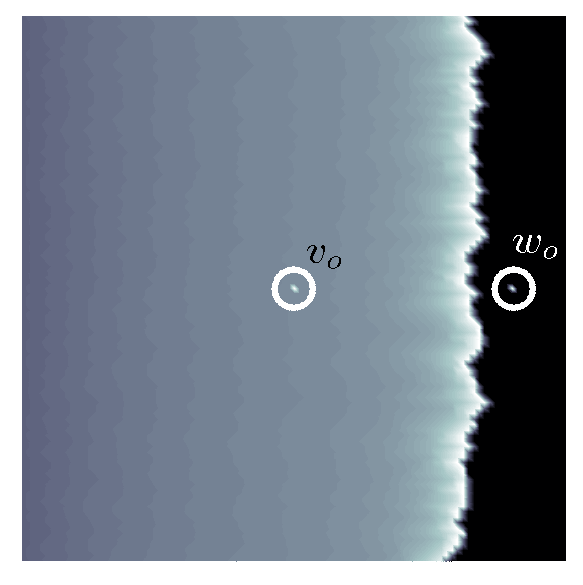
\epsfig{file = ./images/02_chap/Plano_Dinamica.eps,width = 4.5cm} &
%  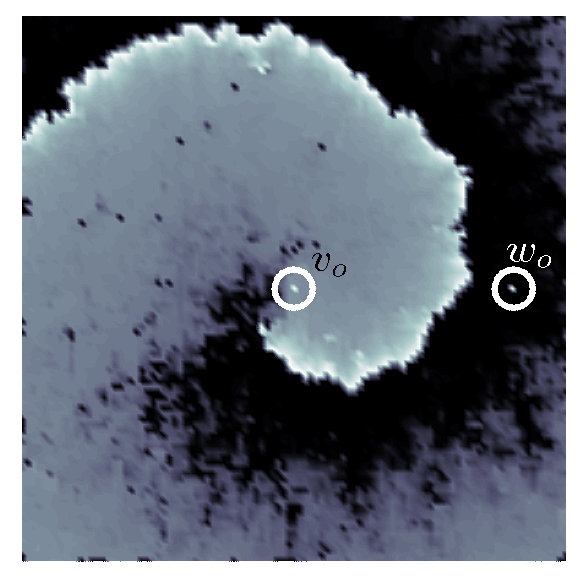
\epsfig{file = ./images/02_chap/Espiral_Dinamica.eps,width = 4.5cm} &
%  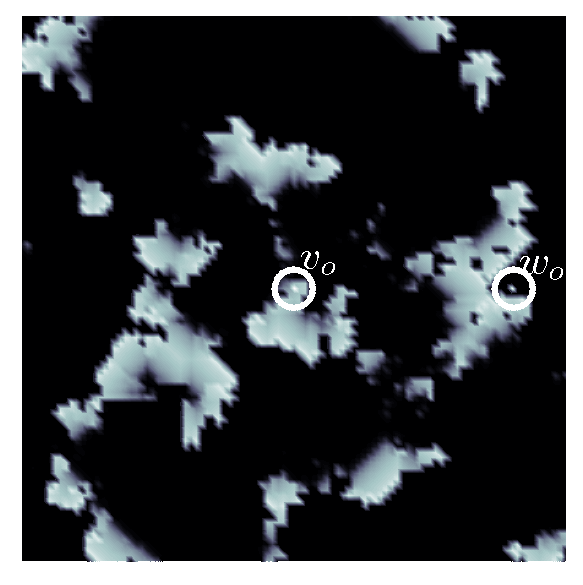
\epsfig{file = ./images/02_chap/Caos_Dinamica.eps,width = 4.5cm}\\
%  (a)  & (b) &  (c)
%  \end{tabular}
%   \caption{ejemplo de dipolos (a) perfectamente correlacionados, (b))
%   parcialmente correlacionados y (c) perfectamente incorrelacionadas .}
%   \label{fig:dinámicas}
% \end{figure}
%
\subsection{Grado de auto-correlación del tejido cardiaco}

% El grado de auto-correlación de una región nos da el porcentaje de dipolos correlacionados dentro del volumen cardiaco. Se cuantifica la relación entre los dipolos del tejido cardiaco, a través del promediado del número de dipolos correlacionados  en cada mapa de intensidades pico.
%
% En este sentido, si la región de auto-correlación es homogénea, podemos  hablar de áreas perfectamente  auto-correlacionadas cuando todos sus elementos están correlacionados entre si, y de áreas  perfectamente incorrelacionadas cuando todos los elementos de  la región no satisfacen el  grado de correlación, es decir su intensidad pico es nula.  Si la región de auto-correlación presenta diferentes intensidades de correlación total, nosotros definimos umbrales de correlación y de esta forma, se  clasifican las dinámicas parcialmente correlacionadas.
%
% En este orden y en función de un umbral de correlación, nosotros definimos la función boleana para todos los elementos del mapa de intensidades pico de correlación, como:
%
% \begin{equation}
%  \boldsymbol{U}(v,w)=
%  \begin{cases}
%     \begin{tabular}{ll}
%         ${1}$ & if ${r}(v,w) > {u}$\\
%         ${0}$ & otherwise
%     \end{tabular}
%  \end{cases}
% \end{equation}
%
%  La intensidad pico de correlación total de los  dipolos  $\mathbf{J}(v_0,t)$ y $\mathbf{J}(w,t)$, esta definido por:
% \begin{equation}
% {r}(v_o,w)  =max{|{R'_{J}}(v_o,w,\tau)|}
% \end{equation}
%
% Donde ${r}(v_o,w)$, puede tomar valores entre 0 y 1, De esta forma, el mapa de intensidades pico de correlación del dipolo $\mathbf{J}(v_0,t)$, contiene  todo los elementos correspondientes  a  ${r}(v_o,w)$,  donde $w$ denota cada uno de los dipolos de $V$. Si ${r}(v_o,w)=0$, decimos que los dipolos  $\mathbf{J}(v_0,t)$ y $\mathbf{J}(w,t)$, están perfectamente  incorrelacionados, cuando  ${r}(v_o,w)=1$, decimos que los dipolos  $\mathbf{J}(v_0,t)$ y $\mathbf{J}(w,t)$ están perfectamente correlacionados. Cuando  $w = v_o$, ${r}(v_o,w)$ es la intensidad máxima de la auto-correlación del dipolo $\mathbf{J}(v_0,t)$, por lo que ${r}(v_o,w)={r}(v_o,v_o)=1$.
%
%
%
%
% Donde $u$ es el umbral de correlación  normalizado  por encima del cual  consideramos que la intensidad pico de correlación total ${r}(v,w)$ es satisfactoria, $u$ varia entre 0 y 1. Si la región de auto-correlación es heterogénea, es de suponer que a mayor valor del umbral de correlación es menor el radio de la región de auto-correlación. De esta manera, el grado de auto-correlación del tejido cardiaco  se puede define como el promedio de la cantidad de  dipolos  correlacionados  para cada $\mathbf{U}(v.w) \in V$.
%
% \begin{equation}
% {T}=\frac{1}{V^2}\int_{VxV}{\mathbf{U}(v,w){dvdw}}
% \end{equation}
%
% En consecuencia, basados en el umbral de correlación,  el volumen  cardiaco se
% caracteriza de acuerdo al grado de auto-correlación,  en donde, en función del
% porcentaje de dipolos que satisfacen la auto-correlación hablamos de  tejido
% correlacionado o incorrelacionado. Si el tamaño de  la región de
% auto-correlación  es equiparado  con el tamaño del tejido observado por el Lead
% Field,  podemos hablar que el tejido cardiaco se aproxima a una dinámica
% perfectamente  correlacionada, por el contrario cuando  el  tamaño  de la región
% de auto-correlación  es significativamente menor que el volumen del  tejido,
% hablamos de dinámicas incorrelacionadas.
%
\subsection{Espectro de señales cardiacas}

% La estimación de la densidad espectral de potencia,   tanto para el  dipolo como
% para las señales cardiacas,  se realiza con el método de Welch.  La resolución
% de la estimación espectral depende  del  número de muestra del  e nventanado y
% del solapamiento del mismo. El cálculo del promedio de periodogramas,  para
% observar la  envolvente espectral en las diferentes resoluciones  de Lead Field
% en cada una de las dinámica simuladas, se realiza con una ventana  Hamming de
% 512  muestras y un solapamiento del 50\%. Para ilustrar la  relación entre los
% espectro de las señales cardiacas del frente de onda plano y su dinámica
% temporal,  nosotros empleamos ventanas Hamming de 2048 muestras para la
% estimación del  espectro de potencia  y observar los armónicos de la señal.
%
% Las señales cardiacas de las tres dinámicas simuladas (frente de onda plano,
% espiral y caos), son sintetizadas en los 8 tamaños de lead Field definidos,
% $A_1$, $A_2$, $A_3$, $A_4$, $A_5$, $A_6$, $A_7$ y $A_8$,. el tiempo total  de
% simulación es de 60 s. Para la estimación del espectro  y  los mapas de
% correlación  se toma un intervalo de 20 s. La  tasa de muestreo de las señales
% sintetizadas es de 500 Hz.
%
% El espectro de las señales cardiacas  en la dinámica perfectamente correlacionada, como se expone en \cite{RequenaSpectral1}, tiene asociado la función de diferencia de tiempos de activación ${\zeta}(v,w)$. Las diferencias de  tiempo son estimadas a partir de los instantes de  despolarización  de los  dipolo $\mathbf{J}(v,t)$ y $\mathbf{J}(w,t)$.  Cuando $v=w  { \zeta}(v,w)=0$. Para  las cuatro resoluciones espaciales de mayor tamaño de LeadField  se generan la funciones de distribución $F_{A_1}(\zeta)$, $F_{A_2}(\zeta)$, $F_{A_3}(\zeta)$, $F_{A_4}(\zeta)$, respectivamente, y constituyen la descripción espacial de los dipolos perfectamente correlacionados.  De esta forma, el espectro  de las señales cardiacas en dinámicas perfectamente correlacionas es expresado por:
%
% \begin{equation}
% S_{C_o}(\omega)=S_{A_o}(\omega) \cdot  S_{J}(\omega)
% \end{equation}
%
% Donde, $S_{A_o}(\omega)$, es la transformada de  Fourier de la funcion de distribución de  tiempos  $F_{A_o}(\zeta)$ y $S_{J}(\omega)$, es el espectro de un  dipolo del  tejido cardíaco. por lo que, el espectro del las  señales cardiacas en el frente de onda plano, depende de la resolución espacial de cada leadField que nosotros definimos. En consecuencia, nosotos calculamos a partir de la funcion de distribución de  tiempos, $S_{A_1}(\omega)$, $S_{A_2}(\omega)$, $S_{A_3}(\omega)$, $S_{A_4}(\omega)$.
%
%
%
\subsection{Espectro de Fuentes Cardíacas}

%
%  The spectrum of a cardiac source, $\boldsymbol{\sigma}(v,w,f)$, $\forall v,w\in
%  V$, corresponds to the collection of the cross-spectra between all pairs of
%  dipoles in $V$, and is defined as
%  \begin{eqnarray}\label{eq:spectrum_source}
%  &&\boldsymbol{\sigma}(v,w,f) =\mathcal{F}[\boldsymbol{\rho}(v,w,\tau)]
%  \nonumber \\
%  &&=\left( \begin{array}{ccc}
%  {\sigma}_{xx}(v,w, f) & {\sigma}_{xy}(v,w, f) & {\sigma}_{xz}(v,w, f) \\
%  {\sigma}_{yx}(v,w, f) & {\sigma}_{yy}(v,w, f) & {\sigma}_{yz}(v,w, f) \\
%  {\sigma}_{zx}(v,w, f) & {\sigma}_{zy}(v,w, f) & {\sigma}_{zz}(v,w, f)
%  \end{array} \right)
%  \end{eqnarray}
%  where the operator $\mathcal{F}[\cdot]$ is applied to
%  $\boldsymbol{\rho}(v,w,\tau)$ on a component-by-component basis. For instance,
%  ${\sigma}_{zy}(v,w, f)$ is $\mathcal{F}[{\rho}_{zy}(v,w,\tau)]$.
%
%  We also define the \emph{total cross-correlation} $R_{J}(v,w,\tau)$ between two
%  cardiac dipoles $\mathbf{J}(v,t)$ and $\mathbf{J}(w,t)$ as the sum of the
%  entries of $\boldsymbol{\rho}(v,w,\tau)$ and the \emph{total cross-spectrum}
%  $S_{J}(v,w,f)$ as the Fourier Transform of $R_{J}(v,w,\tau)$. Mathematically,
%  they can be expressed as
%
%  \begin{eqnarray}
%  S_{J}(v,w,f)  &=&  \mathbf{1}^{T} \boldsymbol{\sigma}(v,w, f)  \mathbf{1}.
% \label{total_spectrum}
% \end{eqnarray}
%
%  Finally, we define the \emph{normalized} cross-correlation
% $\boldsymbol{\hat{\rho}}(v,w,\tau)$ as the matrix of entries
% \begin{equation}\label{eq:normalized_autocorrelation_source}
% \hat{\rho}_{ab}(v,w,\tau) = \frac{{\rho}_{ab}(v,w,\tau)}{\sqrt{{\rho}_{aa}(v,v,0){\rho}_{bb}(w,w,0)}}
% \end{equation}
%  where $a,b\in \{x,y,z\}$, and the \emph{normalized} total cross-correlation
% $\hat{R}_{J}(v,w,\tau)$ as
% \begin{equation}\label{normalized_total_corr}
% \hat{R}_{J}(v,w,\tau)= \frac{R_{J}(v,w,\tau)}{{\underset{\tau}{\max}}\{R_{J}(v,w,\tau)\}}.
% \end{equation}
%
%


\section{Métodos estimación del espectro}
\section{Frecuencia Dominante}

% hablar aca de Fischer  \cite{Fischer07} y de Berenfeld \cite{Berenfeld10},
% \cite{Berenfeld11} ,\cite{Berenfeld07}, \cite{Berenfeld10}

\section{Concluciones}
